\section{Interval Vertex Coloring (IVC)}

\begin{frame}{Vertex Coloring Problem}
  \begin{columns}
    \column{.6\textwidth}
      \begin{itemize}
        \item<1-> Given G(V,E)
        \item<2-> Find a vertex coloring s.t. colors on adjacent vertices differ
      \end{itemize}
      \begin{block}{Formal Definition of VCP given G(V,E)}<3->
        $\text{find} \, f(v):$
        $\forall v\in V:\forall w \, in \, \Gamma(v): f(v) \neq f(w).$
      \end{block}
      
    \column{.4\textwidth}
    \centering
      \null
    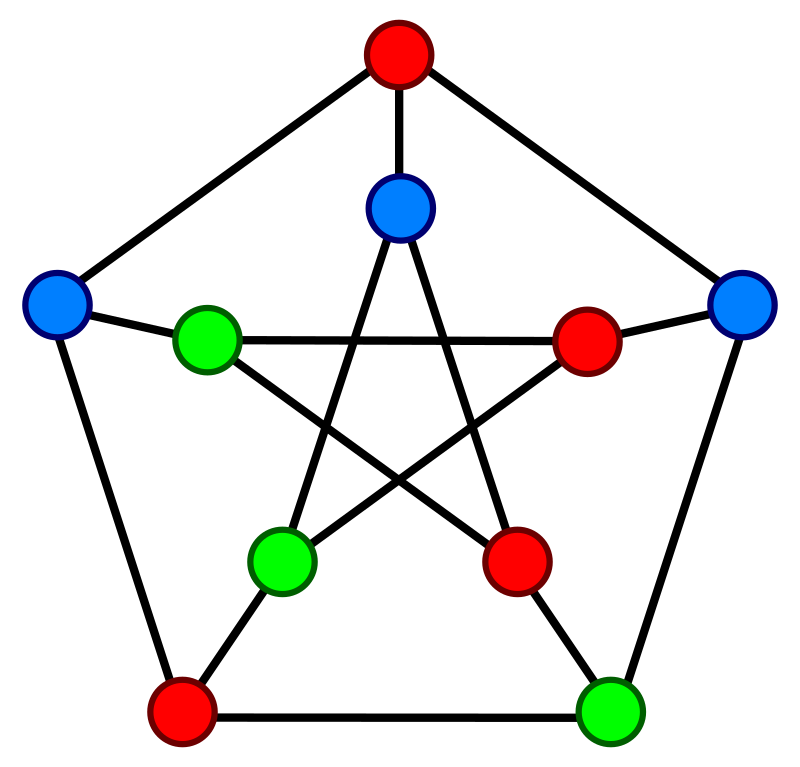
\includegraphics[width=\textwidth]{figures/graph_coloring.png}
    \null
    \centering
      G(V,E)
  \end{columns}
\end{frame}

\begin{frame}{Interval Vertex Coloring (IVC)}
  \begin{columns}
    \column{.4\textwidth}
        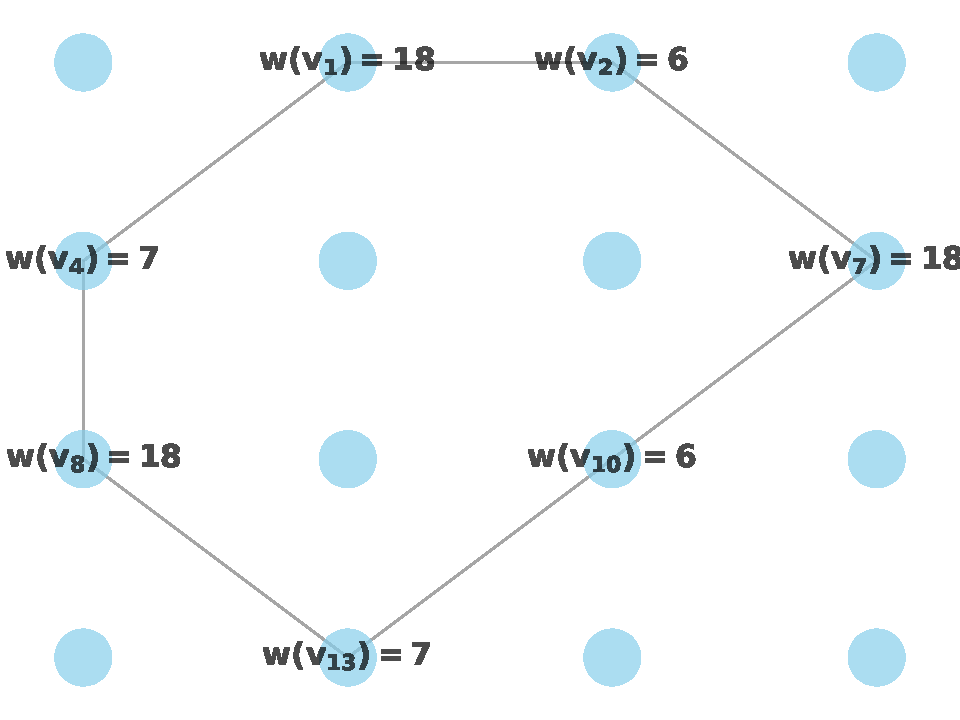
\includegraphics[width=1\textwidth]{figures/ICV0.pdf}<1->
        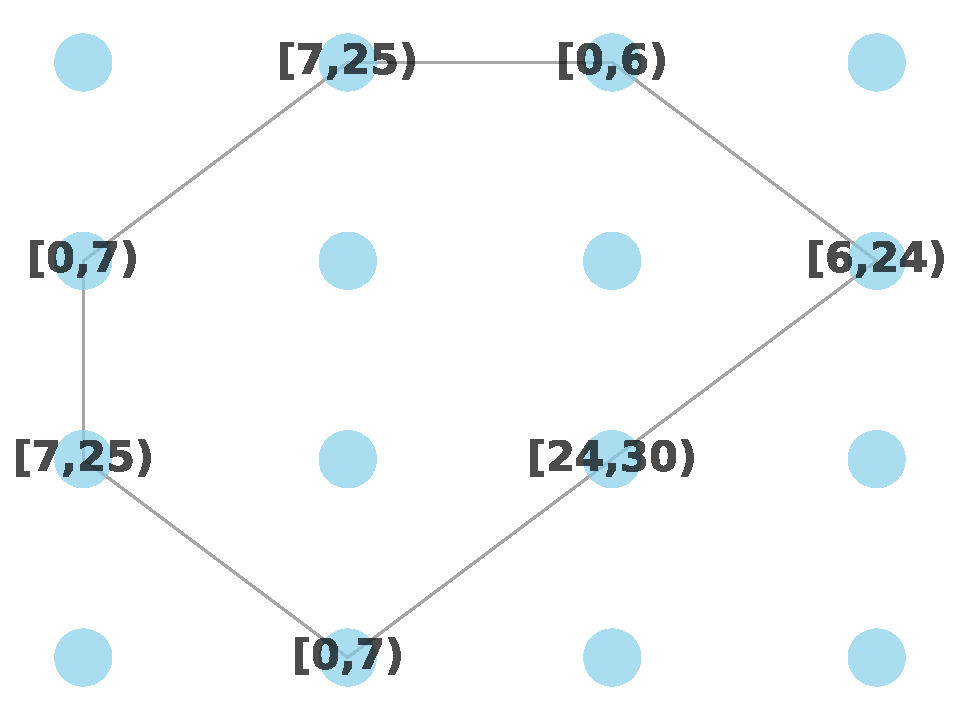
\includegraphics[width=1\textwidth]{figures/ICV1.pdf}<5->
    \column{.6\textwidth}
    \begin{itemize}
    \item<1-> Let G(V,E) be an undirected graph and $w : V \mapsto \mathbb{Z^+}$
    \item<2-> Vertex v is colored with open interval:
    \end{itemize}
    \begin{block}{Vertex v is colored with open interval}<3->
      $[\text{s}(v), \text{s}(v)+w(v))$
    \end{block}
    \begin{block}{Neighboring Vertices must have disjoint color interval}<4->
      $\forall (a, b) \in E, [s(a), s(a) + w(a)) \cap [s(b), s(b) + w(b)) = \emptyset.$
    \end{block}    
  \end{columns}
\end{frame}

\begin{frame}{Formal IVC Problem Definition}
  \begin{block}{Definition:}
    A particular coloring start of G(V,E) is said to use 
    \[ \text{maxcolor}= \max_{v \in V} s(v) + w(v) \hspace{1cm}  \text{colors.}\] 
  \end{block}

  \begin{block}{Optimization Problem Instance:}
    Find a coloring $\text{start}:V \mapsto \mathbb{Z}^+$ that minimizes maxcolor.
  \end{block}

  \begin{block}{Definition}
    The optimal value of maxcolor, i.e. one that comes from a valid minimizer function start,
    is denoted with maxcolor*.
    
  \end{block}
  
\end{frame}
  % \begin{frame}
  %   \begin{columns}[c]

  %     \column{.5\textwidth} 
  %       \begin{itemize}
  %         \item Some text
  %         \item with a picture on the right
  %         \item blah blah
  %         \item more blah blah
  %       \end{itemize}
      
  %     \column{.5\textwidth}
  %       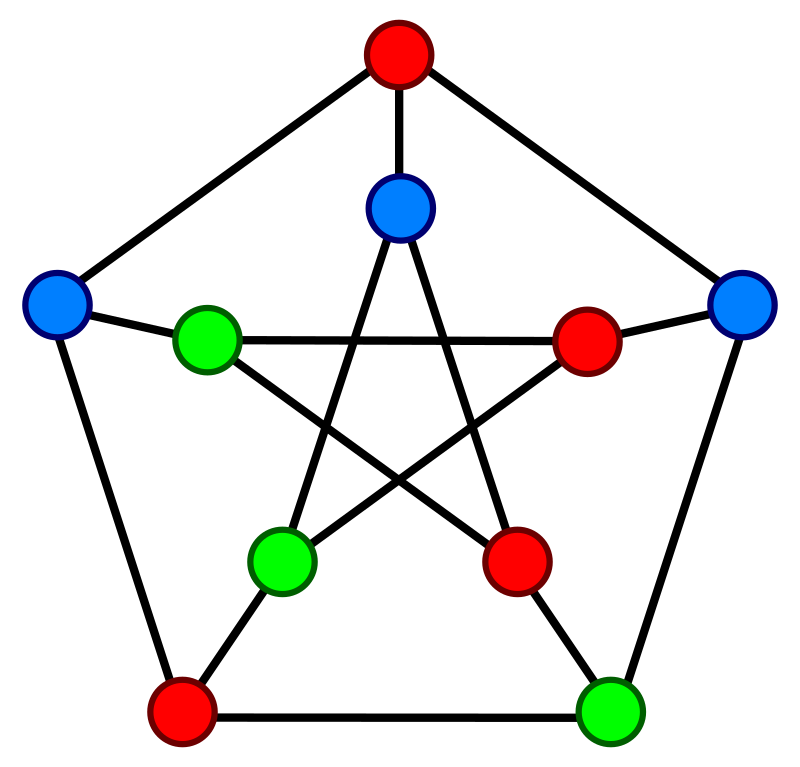
\includegraphics[width=.8\textwidth]{figures/graph_coloring.png}

  %   \end{columns}
  % end{frame}


  \subsection[Paragraphs]{Simple Paragraphs}
  \begin{frame}[fragile]
    \frametitle{Title first category}
    \framesubtitle{Title second category}
    % no deeper title hierarchy provided
  
    Lets see if the citation works in this part \cite{main_paper}. The second paper I use
    should appear in the bibliograph now \cite{kernel_estimation_1} and the third one as well
    \cite{kernel_estimation_2}.
  
    You can cite~\cite{Tan11}. Urls look like this: \url{http://www.google.com/}.
  \end{frame}